\documentclass[11pt,a4paper]{article}

\usepackage{times}
\usepackage{url}
\usepackage{graphicx}

\pagestyle{empty}

\textheight=25cm
\textwidth=15cm
\topmargin=-2cm
\oddsidemargin=0cm

\begin{document}

\begin{center}
  Ole Nielsen \\
  19 Melba Street
  Downer ACT 2602
  M: +61 401 966 202, \ \ \ E: Ole.Moller.Nielsen@gmail.com
  %Jalan Patra Kuningan X, No 3\\
  %Jakarta Selatan 12950, Indonesia \\
  %P: +62 811 820 4637,\ \ \ E: nielso@ausaid.gov.au
\end{center}
\begin{center}
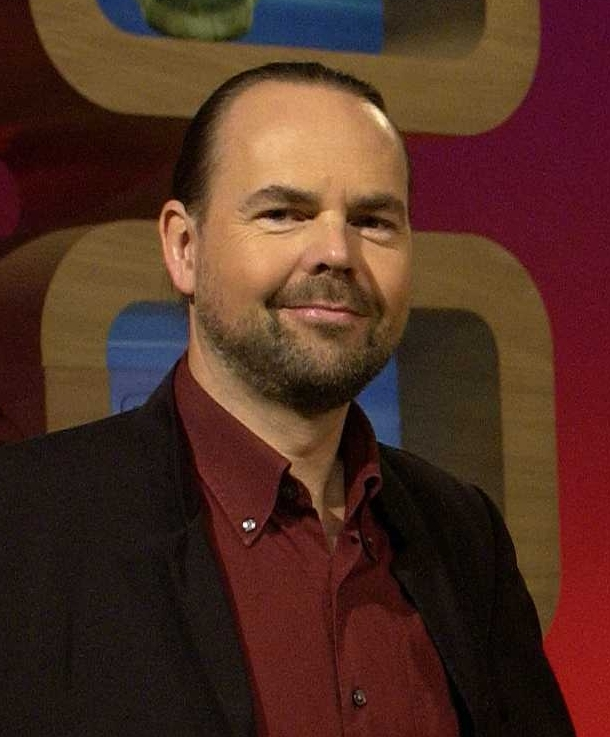
\includegraphics[width=50mm,keepaspectratio=true]{ole.jpg}
\end{center}

\begin{center}
  \hrulefill \\
  {\bf Mission} \\[-0.2cm]
  \hrulefill
\end{center}

\begin{center}
\emph{Focusing on issues that matter.}\\
\emph{Working together to achieve greatness.}\\
\emph{Embracing and driving change.}
\end{center}

\begin{center}
  \hrulefill \\
  {\bf Quotes from colleagues} \\[-0.2cm]
  \hrulefill
\end{center}

\begin{itemize}
  \item Ole has been at the forefront of software development at GA since his arrival in 2003, influencing not only those projects that he worked on directly but others such as the EQRM, a project that has benefited from Ole’s ideas around pair programming, unit testing, version control, issue tracking, documentation, and open-source. He is one of few at GA that can genuinely command respect as a scientist, a software developer and a manager.  He has a contagious level of enthusiasm and a willingness to find agency wide solutions that increase staff productivity in the science divisions. Ole is an inspiration to those of us that have worked with him. %I am stronger at my job courtesy of time spent with Ole.
  \emph{Dr David Robinson, GA, 2014}
  \item Ole’s ideas in 2005 were right at the forefront of best practice and innovation in software development. That he was able to implement those ideas to deliver the highly complex ANUGA software and apply that to assist decision makers understand tsunami inundation risk is a unique achievement. \emph{Gordon Cheyne, Geoscience Australia, 2014}.
  \item Ole is not only an expert at software development; he is equally skilled at working with people, and is remarkable in his ability to build and lead interdisciplinary teams of technical specialists to develop products. This combination of technical and management expertises made Ole the ideal candidate to be seconded for three years to Jakarta to assist in establishing the Australia Indonesia Facility for Disaster Reduction (AIFDR) as part of a GA-AusAID portnership. Ole is extremely well respected by Indonesian colleagues in the technical/science community as well as in the emergecncy management stakeholder community. \emph{Dr John Schneider, GA, 2014}
  \item I use three software packages (PyPar, ANUGA and InaSAFE) that Ole has lead the development of as a core component of my day-to-day work. I use them because they are well-tested, robust open source software packages that are scientifically rigorous and adapted to solve the key science questions I face. I have worked with Ole since 2007 and find his drive and enthusiasm for applying state-of-the-art computational methods to complex scientific problems inspirational. \emph{Jonathan Griffin, Geoscience Australia, 2014}
  \item “Truly outstanding” is the best way to sum up the leadership that Ole has shown in the use of high performance computing and professional software engineering to support a wide range of applications within Geoscience Australia. \emph{GA AGM award 2008}.
  \item Ole’s discipline and demand for high quality software engineering has allowed the tsunami risk modelling team to undertake challenging cutting-edge projects for a number of clients with confidence that our tools can meet varied requirements. \emph{Dr Jane Sexton, Geoscience Australia, 2008}.
  \item Ole almost single handedly championed the idea of GA obtaining a Beuwolf cluster computer, by first developing a small test bed, gathering together a band of users and then being deeply involved in the subsequent business plan, tender, purchase and testing of the new GA system. \emph{Prof Stephen Roberts, ANU Dept Mathematics, 2006}.
  \item It is always great to work with Ole on a project. He brings to the table impressive software engineering skills (I learnt to use unit testing under his influence), impressive scientific and mathematical skills (he incorporated a number of clever ideas into our tsunami simulation code, anuga) and finally and perhaps most importantly great people skills, always motivating and bringing together people with different skills (and personalities) to successfully complete sophisticated projects (the anuga project, the inasafe project). \emph{Prof Stephen Roberts, ANU Dept Mathematics, 2014}.
\end{itemize}

\begin{center}
  \hrulefill \\
  {\bf Career History} \\[-0.2cm]
  \hrulefill
\end{center}

\begin{itemize}
\item {\em Mar 2013 -- Present}: Software Development Manager, Geoscience Australia.
      Oversight of software development, management of 39 staff, responsible for software quality and knowledge management.
\item {\em Mar 2010 -- Mar 2013}: Numerical Modeller, Australia-Indonesia Facility for Disaster Reduction, AusAID, Indonesia.
      Oversight of software engineering and computational infrastructure supporting the Indonesian government disaster management agency in better planning and decision making.
\item {\em Mar 2003 -- Mar 2010}: Senior Computational Scientist, Geoscience Australia.
      Research, development and application of natural hazard models. In particular, leading the development of ANUGA hydrodynamic modelling and its application in tsunami impact modelling.
\item {\em Sep 2003 -- Dec 2003}: Visiting Professor,
      Department of Mathematics,
      Suranaree University of Technology, Nakhorn Ratchasima, Thailand. Teaching PhD course in
      High Performance Computing.
\item {\em Nov 1998 -- Feb 2003}: Research Fellow,
      School of Mathematical Sciences, Australian National University.
      Research in enterprise datamining.
\item {\em Mar 1998 -- Oct 1998}: Scientific Computing Consultant \\
      UNI$\bullet$C, Danish Computing Centre for Research and Education.\\
      Design and development of parallel image analysis algorithm.
\end{itemize}

\pagebreak
\begin{center}
  \hrulefill \\
  {\bf Education} \\[-0.2cm]
  \hrulefill
\end{center}

\begin{itemize}
\item Doctor of Philosophy (May 1998) \\
{\bf Technical University of Denmark} \\
Department of Mathematical Modelling  \\
Thesis: ``Wavelets in Scientific Computing''\\
%Available at {\tt http://datamining.anu.edu.au/\~{}ole} \\
%Grade Point Average: 11.0/13    %All 11's + one A

\item  Master of Science (November 1993) \\
{\bf Roskilde University, Denmark} \\
Department of Computer Science \\
Thesis: ``DISCO -- DIScrete and COntinuous simulation''\\
%Grade Point Average: 11.4/13  %(10.5 + 12 + 11 + 12)/4

\item  Batchelor of Science (June 1990) \\
{\bf Roskilde University, Denmark} \\
Department of Mathematics \\
%Grade Point Average: 11.5/13  %(10+13)/2
\end{itemize}

\begin{center}
  \hrulefill \\
  {\bf Some achievements} \\[-0.2cm]
  \hrulefill
\end{center}

\begin{itemize}
  \item Built cohesive team of almost 40 software developers following centralisation of software development in Geoscience Australia and implemented agreed quality measures and development standards for the main development languages in use in the organisation. I lead the increased focus on Continuous Delivery, Open Source, Test Automation and Cloud Computing as well as day to day people management and conflict resolution.
  \item Lead the development of a novel and user friendly application for rapid and reproducible estimation of impact from natural disasters called InaSAFE which is available at \url{www.inasafe.org}.
  Version 1.0 was publicly and officially launched at the Asian Ministerial Conference on Disaster Risk Reduction in October 2012 and shown to the president of Indonesia as the centrepiece of Australian Indonesian cooperation in Disaster Management. InaSAFE is currently being provided to local and national disaster managers in Indonesia. The World Bank who is a partner in this project is building web applications based on InaSAFE for use world wide.
  InaSAFE won the Black Duck prize for most promising projects of 2012. % \url{http://www.blackducksoftware.com/news/releases/black-duck-announces-2012-open-source-rookies-year-winners}
  \item The ANUGA hydrodynamic modelling project which is a sophisticated open source software model written in Python and C, that has underpinned all tsunami inundation modelling in Australia. Under my leadership, this project lead to two AGM team awards: 2006 (Capability) and 2007 (Influence); was featured in 2009 in a special episode on the Australian TV program The New Inventors \emph{Dealing With Disasters} and attracted the Emergency Management Australia "Safer Communities Award" in 2005 and 2007 as well as the "Asia-Pacific Spatial Excellence Award" in 2007. ANUGA was developed as a strongly test driven project (now with almost 1,000 unit tests) and a comprehensive regression test suite of physical validation examples. ANUGA was released as Open Source in December 2006 (the first from GA) and has since then had over 16,000 downloads and is now used widely outside the organisation - e.g.\ for urban flood modelling: \url{http://en.wikipedia.org/wiki/ANUGA_Hydro}
  %\item A new modelling capability, ANUGA, that can simulate
  %impacts of tsunami, storm surge or flood disasters on the built environment.
  %This work was awarded the Emergency Management Australia "Safer Communities Award" in 2005 and 2007 as well as the
  %Asia-Pacific Spatial Excellence Award in 2007.
  %More information about the ANUGA project is available at \url{http://en.wikipedia.org/wiki/ANUGA_Hydro}
  \item A corporate high performance computing capability in my organisation.
  This involved building a prototype parallel Linux cluster, developing and presenting the business case to the
  senior management team, setting up a corporate wide special interest group, managing the installation process
  from tender to final acceptance testing.
  \item Influencing my workplace to take up modern software development methodologies and practices that
  have improved the quality, speed and audit trail of corporate software.
  \item A binding for the Message Passing Interface (MPI) for the Python programming language.
  Pypar is open source, used widely in the scientific community (bio-informatics, health and datamining and modelling) and underpins projects such as ANUGA, python-FALL3D, URS-TSUNAMI and EQRM.
  Pypar is available at \url{http://code.google.com/p/pypar}
  \item The development of a WEB-enabled
  data exploration tool online analysis of large Health care databases
  at the Health Insurance Commission. This involved datamining and record linkage of about 80 million
  MBS claims and 50 million PBS claims and required the development of special purpose software to
  handle these volumes.
  %\item Designed and developed an open software library for data mining
  %of large relational databases using the scripting language Python
  %This library is successfully used for fast, interactive access to large
  %databases at the Australian National University (ANU) and
  %Commonwealth Science and Industrial Research Organisation (CSIRO).
  %\item Developed database of currently 0.5 million
  %GPS coordinates searchable by proximity to a given location
  %and by optional keywords. The search engine is fast
  %due to data base tables dynamically organised in a tree structure.
  %Wrote WEB front end for searching, retrieving and uploading GPS waypoints
  %using the GPS search engine.
  %\item Successfully implemented and applied a wavelet based algorithm
  %for surface fitting of high-dimensional data for use in predictive modelling.
  \item Developed vector-parallel fast wavelet transforms
  for the Fujitsu scientific software library.
  % at the Australian National University.
  The implementation was accompanied by a performance model that
  predicted both sequential and parallel actual performance.
  About 80 \% of peak performance on one processor was achieved,
  and the parallel efficiency was {\em independent} of the problem size
  as well as the number of processors.
  \item Developed an efficient algorithm for
  wavelet transforms of circulant matrices
  and various operations on them.
  Exploiting the particular structure of this problem
  reduced the storage requirements as well as the algorithmic complexity
  from {\em quadratic} to {\em linear} in the number of non-zeros.
  %\item Did the initial analysis, design, and architecture evaluations
  %towards the parallelisation of a medical image analysis algorithm.
  %\item Published an easy-to-understand wavelet tutorial
  %in IEEE Computer Applications in Power, Volume 12, Number 1, January 1999.
  %\item Have given technical and scientific presentations at
  %various institutions and conferences including
  %International Disaster Reduction Conference (Switzerland 2006);
  %UNESCAP High Level Technical meeting on Tsunami Disasters (Thailand 2005);
  %Australian Earth Quake Engineers annual meeting (GA 2006), Dynamic Earth Conference (ANU 2006),
  %Computational Techniques and Applications Conferences (CTAC 1999, 2006);
  %Modelling and Simulations (MODSIM 2005), Ninth Internal Python Conference (Californa 2001),
  %Australian Epidemiological Association (Sydney); NSW Health; IBM Yorktown heights (USA);
  %St Catherine's College, Oxford (UK); Umeaa University (Sweden);
  %UNI$\bullet$C (Denmark); and many more.
\end{itemize}


\begin{center}
  \hrulefill \\
  {\bf Selected publications} \\[-0.2cm]
  \hrulefill
\end{center}

\input{cv_publ.sub}



\end{document}

